%!TEX root = ../template.tex
%%%%%%%%%%%%%%%%%%%%%%%%%%%%%%%%%%%%%%%%%%%%%%%%%%%%%%%%%%%%%%%%%%%%
%% chapter4.tex
%% NOVA thesis document file
%%
%% Chapter with lots of dummy text
%%%%%%%%%%%%%%%%%%%%%%%%%%%%%%%%%%%%%%%%%%%%%%%%%%%%%%%%%%%%%%%%%%%%

\typeout{NT FILE chapter4.tex}%

\chapter{Background}
\label{cha:background}

In this section, the technology behind the development and deployment of a microservices-based
application system will be described using the underlying design principles.

The technology underlying the development and deployment of microservices-based applications will be described in this section:

\section{Microservices} % (fold)
\label{sec:microservices}

Microservices \cite{microservices, microservices2017tenets, microservicesTomorrow} are an architectural style in which software is developed using self-contained components that
communicate with one another via standardized interfaces and lightweight mechanisms.
These services segregate fine-grained business functionalities and can be independently deployed, scaled, and tested by automated mechanisms.
There is virtually no centralized management, and each service may be written in a different programming language and employ a different data storage technology.

\paragraph{}

To understand the microservice style it's useful to compare it to the monolithic style:
A monolithic application is built often using the Model-View-Controller (MVC) pattern ~\cite{mvc}, which is composed by three parts:
The view, a client-side user interface composed of HTML pages and Javascript that runs in the user's browser;
The model, a relational database management system;
The controller, a server-side application that handles requests, retrieves and updates data from the database, executes domain logic,
and populates the views that are sent to the browser.

\paragraph{}

The server-side application is a monolith a single logical executable, in which all logic for handling requests runs as a single process,
different domains of the application are divided into classes, functions, and namespaces by utilizing the basic features of a programming language.

When large monolithic applications must scale while maintaining a high level of availability, they become a source of frustration:
Scaling the server-side application involves scaling all the application functionalities, rather than the functionalities that require greater resources;
Any small change made to the server-side application, involves building and re-deploying the entire monolith;

\begin{figure}[htbp]
    \centering
    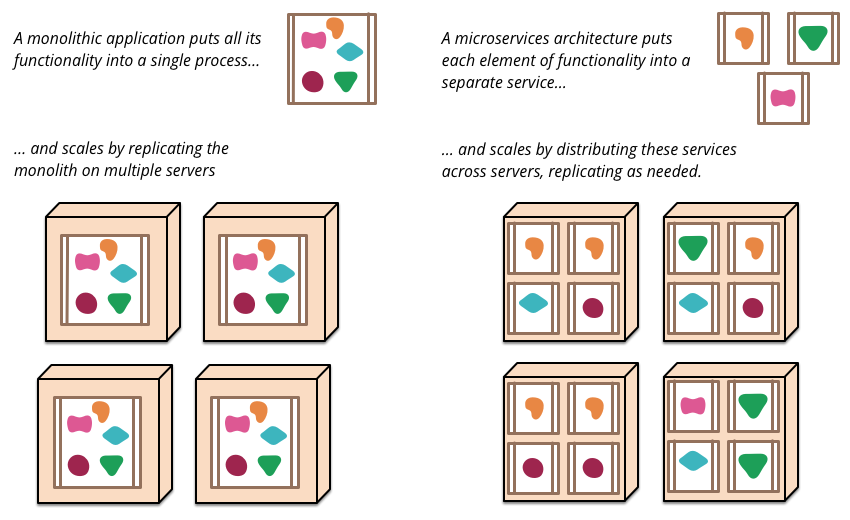
\includegraphics[height=3in]{microVSmono}
    \caption{Monoliths and Microservices \cite{microservices}}
    \label{fig:monoliths and microservices}
\end{figure}

The requirements of system scalability, high availability, and continuous delivery are addressed in different microservice architectural characteristics.

\paragraph{Componentization}

In contrast to monoliths, which achieve componentization solely via the use of libraries and programming language capabilities,
microservices achieve componentization primarily through the division of different business domains and functionalities into distinct executables
that are exposed as services.

While this componentization approach helps to enforce component's encapsulation via more explicit component interfaces,
its primary benefit is that services become independently deployable.
This feature helps to fulfill the requirements of system scalability and high availability by
making different components scalable across multiple nodes and limiting cascading errors via the replication and isolation of components.

\paragraph{Decentralized Data Management}

While monolithic applications typically use a single logical database for persistent data, microservices provide greater flexibility, fault tolerance,
and scalability by allowing each service to manage its own database, which can be a different instance of the same database technology or a completely different database system.
Decentralizing data responsibility across services has implications for the implementation of cross-domain operations affecting multiple resources.
The common approach for dealing with the problem of consistency when updating multiple resources in a database system is to use transactions.
Building and maintaining applications that employ distributed transactions is notoriously difficult; as a result,
microservice architectures advocate for transaction-less service coordination while acknowledging
that consistency will be only eventual and that divergence must be addressed with compensating operations.

\paragraph{Inter-process Communication Strategies}

\citeauthor{microservices}, a well-known author in the context of microservices, advocates what he calls ''smart endpoints and dumb pipes'' for microservices communication.
Enterprise Service Buses (ESB) \cite{esb} were previously frequently used in service-oriented architecture (SOA) systems,
and it was common to incorporate orchestration and transformation logic into the communication infrastructure,
making the pipe ''smart''. There were multiple problems with this approach:
the tooling was complex and expensive, and it was difficult to troubleshoot when problems occurred in production environments.

The reverse approach has been adopted with microservices,
where services own their domain-centric logic ''smart endpoints'' and use ''dumb pipes'' as a transport method.
The majority of communication between microservices is done via request/response-based communication or event-driven messaging.
Because these two methods have such dissimilar properties, it's important to weigh their strengths, and the scenarios that call for each.

Request/response-based communication protocols are typically suited for synchronous settings,
where the client contacts one receiver at time and needs the response before it can continue.
In this approach there is a clear control of the flow,
there is a service that plays the role of orchestrator and determines the sequence of operations to be performed in other services.
The HTTP and RPC protocols are the most widely adopted protocols that follow this approach.

Event-driven messaging communication protocols are suited for asynchronous settings,
where the client publishes a message to multiple receivers and can process the responses at a later time.
In this approach there is no orchestrator, each service knows their role and what to do based on events that occurred.
The main disadvantage of this strategy is that consistency is not guaranteed when multiple services consume events and one of them fails.

\paragraph{Evolutionary Design}
When decomposing a software system into components, we must decide how to divide the pieces.
The concept of independent replacement and upgrade-ability are critical properties when designing a component.
The disadvantage of incorporating components into services is that we must be concerned about changes to one service breaking its consumers.
The traditional integration approach is to attempt to resolve this issue through the use of versioning.
In the context of microservices, versioning entails the maintenance of multiple deployments of the same service in distinct versions.
We can minimize the use of versioning by designing services in such a way that they are as tolerant as possible to supplier changes,
utilizing techniques such as Domain-Driven Design (DDD) \cite{ddd}.
DDD is a software design approach that decomposes a complex system into multiple autonomous bounded contexts,
where all the structure and language of software (class names, class methods, class variables) match the business domain.

\section{Microservice Lifecycle Management} % (fold)
\label{sec:microservice_lifecycle_management}

To run microservices in the cloud, we need two essential ingredients a method for packaging and isolating services,
and a management system capable of provisioning physical hardware to support them.

\paragraph{}

The isolation of services is accomplished through resource virtualization in one of two ways: containers or virtual machines (VM).

Containers provide the most efficient approach because unlike VMs, containers share the host system’s kernel with other containers.
VMs virtualize an entire machine down to the hardware layers, while containers only virtualize software layers above the operating system level.

Docker \cite{docker} is the most popular container technology. It is built on top of the following technologies: Kernel namespaces, Cgroups, Copy-on-write File system.
\begin{itemize}
    \item Namespaces: Isolate the kernel resources (e.g.\ processes, filesystem, users, network stacks) used by each container.
    \item Cgroups: Isolate the hardware resources used by each container.
    \item Copy-On-Write File system: Allows several containers to share common data.
\end{itemize}

Additionally, Docker provides a mechanism for packaging code and its dependencies, referred to as container images.
A container image is a lightweight, standalone executable package of software that contains all the components necessary to run an application: code, libraries, runtime and settings.

\paragraph{}

The management of services can be accomplished with the use container orchestration technologies.
Container orchestration eliminates many of the manual processes involved in the management of distributed systems.
Some popular options used for the lifecycle management of services are Docker Swarm \cite{docker2016swarm} and Kubernetes \cite{kubernetes}.

Kubernetes \cite{kubernetes} is an open-source container orchestration system that evolved from Google's Borg and Omega projects \cite{burns2016borg}.
Kubernetes is an ambitious platform. It manages the deployment, management, scaling, and networking of containers of distributed systems across a wide range of environments
and cloud providers.

This means ensuring that all containers used to execute various workloads are scheduled to run on physical or virtual machines,
while adhering to the deployment environment's and cluster configuration's constraints.
Any containers that are dead, unresponsive, or otherwise unhealthy are automatically replaced.
Additionally, Kubernetes also provides a control plane to monitor all running containers.

Kubernetes accomplishes this through a well-defined, high-level architecture that encourages extensibility:

\begin{itemize}
    \item Pod: Encapsulates an application's container (or multiple containers),
    storage resources, haves a unique network IP address, and provides configuration options for the container(s).
    \item Service: Is an abstraction which defines a logical set
    of Pods and a policy by which to access them.
    \item Volume: Is a directory which is accessible to the
    Containers in a Pod.
    \item Namespace: Provide a scope for names. Names
    of resources need to be unique within a namespace, but not
    across namespaces.
    \item Deployment: Describes the desired state of the system. The
    Deployment Controller changes the actual state to the desired
    state at a controlled rate.
    \item ReplicaSet: Ensures that a specified number of pod replicas
    are running at any given time.
    \item DaemonSet: ensures that all (or some) Nodes run a copy of
    a Pod.
    \item StatefulSet: Is used to manage stateful applications.
\end{itemize}

Kubernetes is a more sophisticated container management system than Docker Swarm.
Docker Swarm is only compatible with Docker, whereas Kubernetes is compatible with other container services.
In comparison to Swarm, Kubernetes is more difficult to deploy and manage, however is said to be more scalable.

\section{Contract Evolution in MicroService Architectures} % (fold)
\label{sec:contract_evolution_in_microservice_architectures}

The evolution of a microservice contracts while ensuring their soundness and
avoiding heavy adaptation processes due to service redeploying is demonstrated to be possible by \citeauthor{seco2020robust} \cite{seco2020robust}.
The proposed approach to microservice contract evolution \cite{seco2020robust} makes use of a global deployment manager component that is responsible for managing module references,
as well as dynamically generated proxies that are capable of adapting messages exchanged between modules when contracts mismatch.
The following example demonstrates the mechanism:

\paragraph{}

\begin{figure}[htbp]
    \centering
    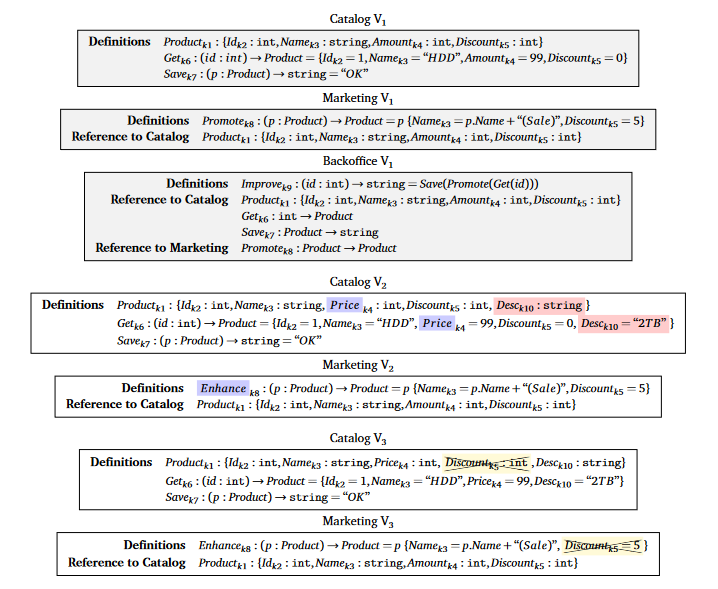
\includegraphics[height=5in]{adapter_example}
    \caption{Evolution of modules Catalog, Marketing, Backoffice \cite{seco2020robust}}
    \label{fig:evolution_of_modules}
\end{figure}

Consider the marketing system shown in Figure ~\ref{fig:evolution_of_modules} that comprises three distinct modules: Catalog, Marketing, and BackOffice.
These three simple modules combined, form a triangle of dependencies, complex enough to demonstrate the proposed mechanism.
Please note that the Catalog module is a producer, whereas the Marketing module is a producer and a consumer.

Each module has a unique name, a collection of type and function definitions, and a set of type and function references.
If a producer module exposes definitions, they can be used by other consumer modules via an explicit reference.
Each programming element is accompanied by an immutable and unique key; for instance – the key of type ''Product'' is k1.
These keys enable elements to be identified even after they have been renamed or reinstated.

Initially, we have a system composed of a collection of services,
each of which hosts an instance of one of the deployed modules shown in grey in Figure ~\ref{fig:evolution_of_modules}.
The reference definitions indicate their interactions.

\paragraph{}

In a second phase, we develop version 2 of the Catalog and Marketing modules independently.
In module Catalog, we rename the element ''Amount'' to ''Price'' and add the attribute ''Desc'', while in module Marketing, we rename ''Promote'' to ''Enhance''.
The module BackOffice has not been modified at this point and will become out of sync with the other modules.
In Figure ~\ref{fig:evolution_of_modules}, the newly added and modified elements are highlighted in red and blue, respectively.

\paragraph{}

In a third phase, Catalog version 3 is created, with the attribute ''Discount'' of the element ''Product'' removed.  (Figure ~\ref{fig:evolution_of_modules}).
This version cannot be deployed in conjunction with version 2 of Marketing, as the attribute is used by the function ''Enhance''.

We can deploy both modules together if we modify the definition of ''Enhance'' to remove the use of the attribute ''Discount'', resulting in version 3 of Marketing.
Additionally, we could deploy version 3 of Marketing first and then version 3 of Catalog, but not vice versa.
Besides this, in the reference to catalog we are permitted to retain the attribute ''Discount'' in the definition of the type ''Product''.
As long as the attribute is not used, correctness is guaranteed.
In Figure ~\ref{fig:evolution_of_modules}, the elements that have been removed are highlighted in yellow.

As illustrated by the multiple versions of the modules,
the proposed system is capable of overcoming differences in contract definitions by utilizing a communication protocol
that adapts automatically to the following types of changes:

\begin{itemize}
    \item \textbf{Adding new attributes to a record type} The ''Desc'' attribute was added to Catalog, and thus the data returned by this module will contain values for this attribute.
    Other modules will retain this data (as unknown attributes) in order to ensure that no data is lost when crossing services boundaries.
    \item \textbf{Renaming functions} The ''Promote'' function in module Marketing has been renamed to ''Enhance'', which will have an effect on the endpoints exposed by the service.
    At runtime, the proxy is dynamically generated to use the actual endpoint name when issuing calls, avoiding the need to update and redeploy the service Backoffice.
    \item \textbf{Removing unused attributes or functions.} Unused elements do not require explicit adaptation.
\end{itemize}

Traditional approaches, such as HTTP, are insufficiently robust to handle these types of changes, effectively rendering them breaking changes.

For instance, renaming functions results in the modification of remote URIs, and changing the name of an attribute may result in data loss.
By contrast, with the presented approach, such changes are permitted without compromising module compatibility.

This adaptive approach enables gradual module deployment of the referenced modifications without halting the entire system, avoiding data loss and misinterpretations.

Experimental data \cite{seco2020robust} collected over a five-year development period on the evolution of three large software factories each containing over 1000 modules
(a raw dataset containing 8889 production deployments with a total of 23986 signature changes)
indicates that this approach would be effective in an average of 57\% of deployments that would require adaptation and recompilation.